\section{Assumptions}
In this section we are going to describe the various assumptions that were made in order to solve this assignment. 
\subsection{Navigation Assumptions}
For moving around the robot we have decided to use 10 waypoints.
To be precise, such waypoints are described with the following image :
\begin{center}
    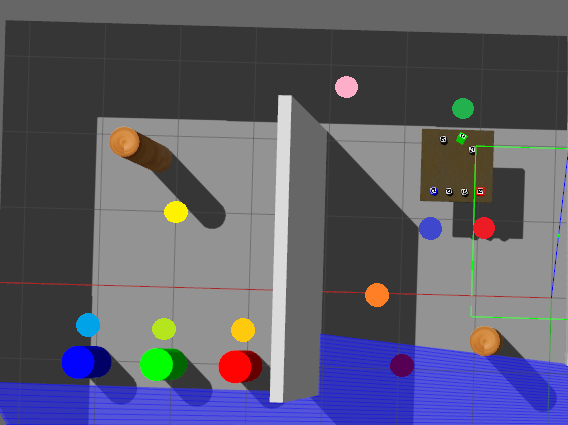
\includegraphics[scale = 0.85]{images/assumptions/waypoints-short.png}    
\end{center}
    Notice that : 
    \begin{itemize}
    \item \textbf{\textcolor{red}{red}}, \textbf{\textcolor{blue}{blue}}, \textbf{\textcolor{ForestGreen}{green}}, \textbf{\textcolor{pink}{pink}}, \textbf{\textcolor{orange}{orange}}, \textbf{\textcolor{Purple}{dark violet}} and \textbf{\textcolor{yellow}{yellow}} colored waypoints are used for the solution of the Assigment with and without the extra point part.
    \item \textbf{\textcolor{DodgerBlue}{light blue}}, \textbf{\textcolor{green}{light green}} and \textbf{\textcolor{Orange}{light orange}} colored waypoints are used in addition to the previous for solving the part of the Assigment without extra points.
\end{itemize} 
Moreover, the meaning of the single waypoints is the following :
\begin{itemize}
    \item \textbf{\textcolor{red}{red}} waypoint : is the pick-position for the red cube.
    \item \textbf{\textcolor{blue}{blue}} waypoint : is the pick-position for the blue hexagon.
        \item \textbf{\textcolor{ForestGreen}{green}} waypoint : is the pick-position for the green tetrahedron.
    \item \textbf{\textcolor{Purple}{dark violet}} waypoint : is the waypoint used to avoid that the robot try to go through the circular obstacle after the corridor and the wall of the room.
    \item \textbf{\textcolor{orange}{orange}} waypoint : is the waypoint used only after having picked the red cube or blue hexagon for avoiding to hit the table if the robot tries to move directly from \textbf{\textcolor{red}{red}} or \textbf{\textcolor{blue}{blue}} waypoints to the \textbf{\textcolor{pink}{pink}} waypoint.
    \item \textbf{\textcolor{pink}{pink}} waypoint : is the waypoint reached after having picked an object. Notice that when the robot picks the green tetrahedron it is reached from the \textbf{\textcolor{ForestGreen}{green}} waypoint, while when the robot picks the blue hexagon or the red cube it is reached from the \textbf{\textcolor{orange}{orange}} waypoint.
    \item \textbf{\textcolor{yellow}{yellow}} waypoint : is the docking position used for obtaining the centers of the place tables (It is used both for solving the Assigment in the extra point and no extra point version, but in the no extra point version it determines only the centers of the cylindrical tables for building the pose of where to place the object, while in the extra version of the assigment, in addition to that it is used also for determining the position of the table of where to place the current picked object).
    \item \textbf{\textcolor{DodgerBlue}{light blue}} waypoint : is the position of the robot for placing the blue hexagon in the corresponding cylindrical place-table of blue color. (Used only for no-point extra version of the Assigment)
    \item \textbf{\textcolor{green}{light green}} waypoint : is the position of the robot for placing the green tetrahedron in the corresponding cylindrical place-table of green color. (Used only for no-point extra version of the Assigment)
    \item \textbf{\textcolor{Orange}{light orange}} waypoint : is the position of the robot for placing the red cube in the corresponding cylindrical place-table of red color. (Used only for no-point extra version of the Assigment)
\end{itemize}
% ------------------------------------------------------------------------
% MANIPULATION ASSUMPTIONS
% ------------------------------------------------------------------------
\subsection{Manipulation Assumptions}
The assumptions made in the manipulation part are mainly concerned the following aspects: intermediate pose of TIAGo's arm and gripper after the pick phase, the different picking poses of the objects and the approach pose used to pick the objects. We provide also some images for better understanding our assumptions:
\begin{enumerate}
    \item We used a predefined pose for TIAGo's arm and gripper before and after the pick phase, so that it is away from the planning scene in front of the robot  and does not obstruct its view. We have chosen a slightly elevated side position, as can be seen in the figure:
    \begin{center}
    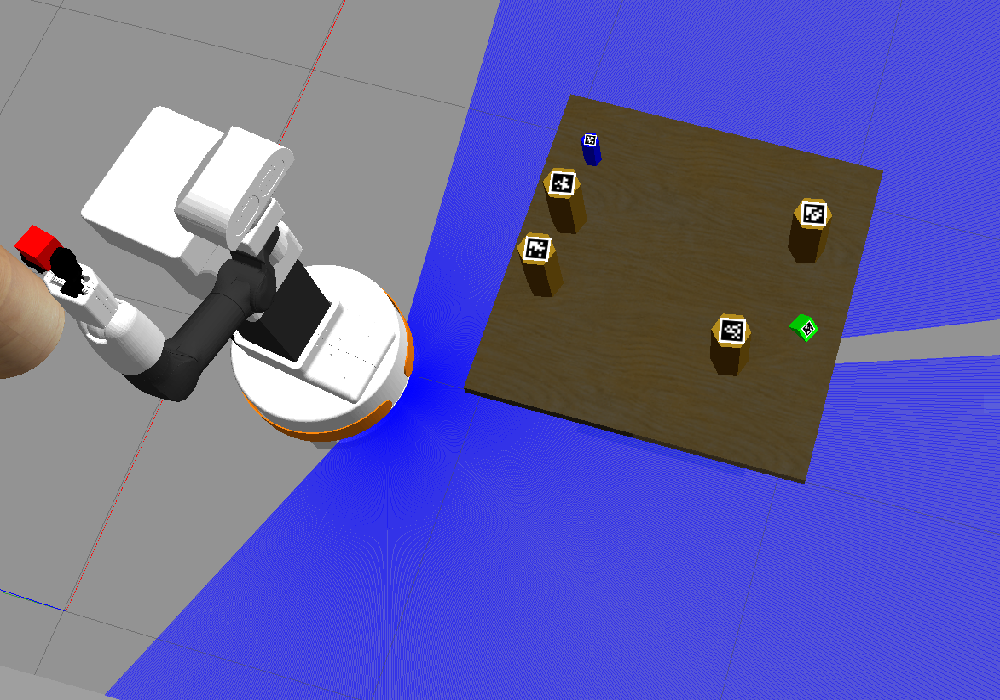
\includegraphics[scale = 0.3]{images/manipulations/afterPick.png}    
    \end{center}    
    
    \item Next, we engineered a specific picking pose for each object, in particular, a pose from above for the green tetrahedron and the red cube, and a side one, instead, for the blue hexagon, as can be seen in the figures:    
    \begin{figure}[H]
        \begin{minipage}{0.33\textwidth}
            \centering
            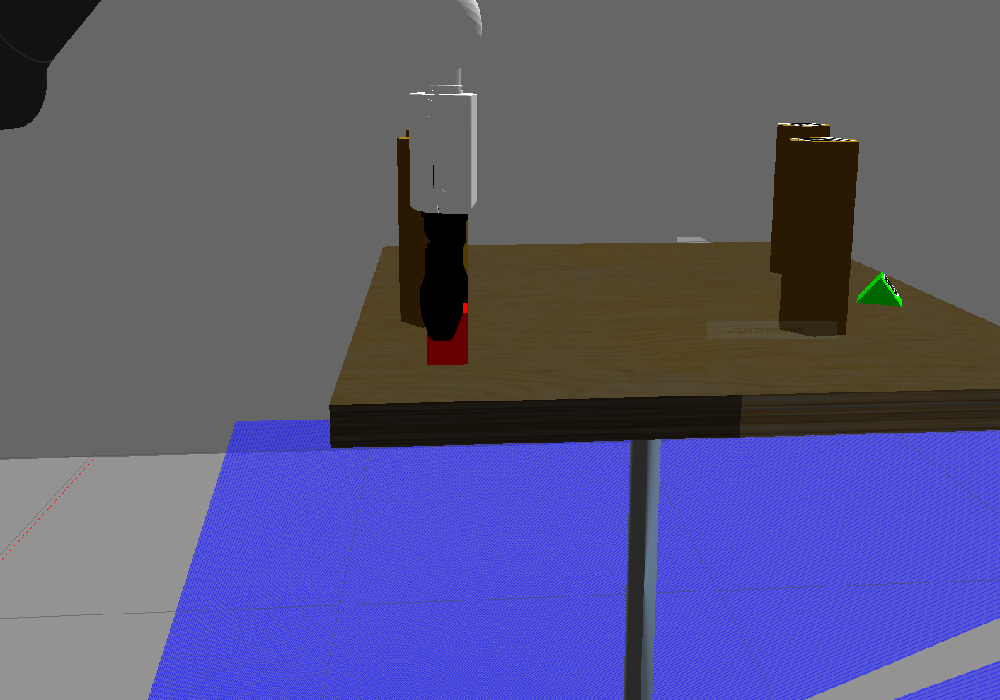
\includegraphics[scale = 0.18]{images/manipulations/pick.png}
            \captionof{figure}{Pick red}
        \end{minipage}
        \begin{minipage}{0.33\textwidth}
            \centering
            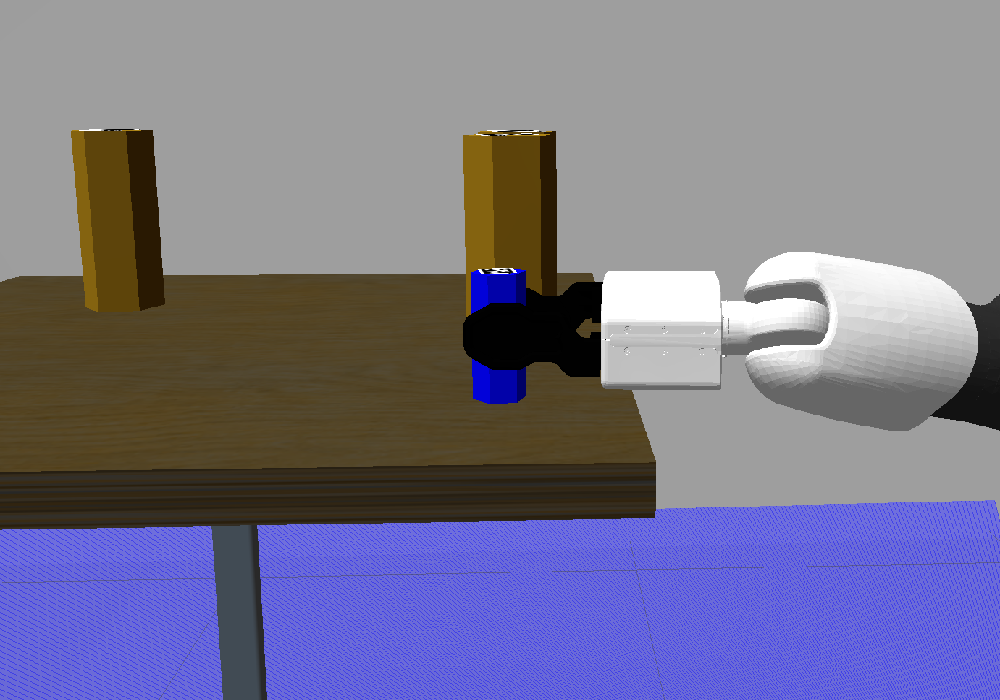
\includegraphics[scale = 0.18]{images/manipulations/pickBlue.png}
            \captionof{figure}{Pick Blue}
        \end{minipage}
        \begin{minipage}{0.33\textwidth}
            \centering
            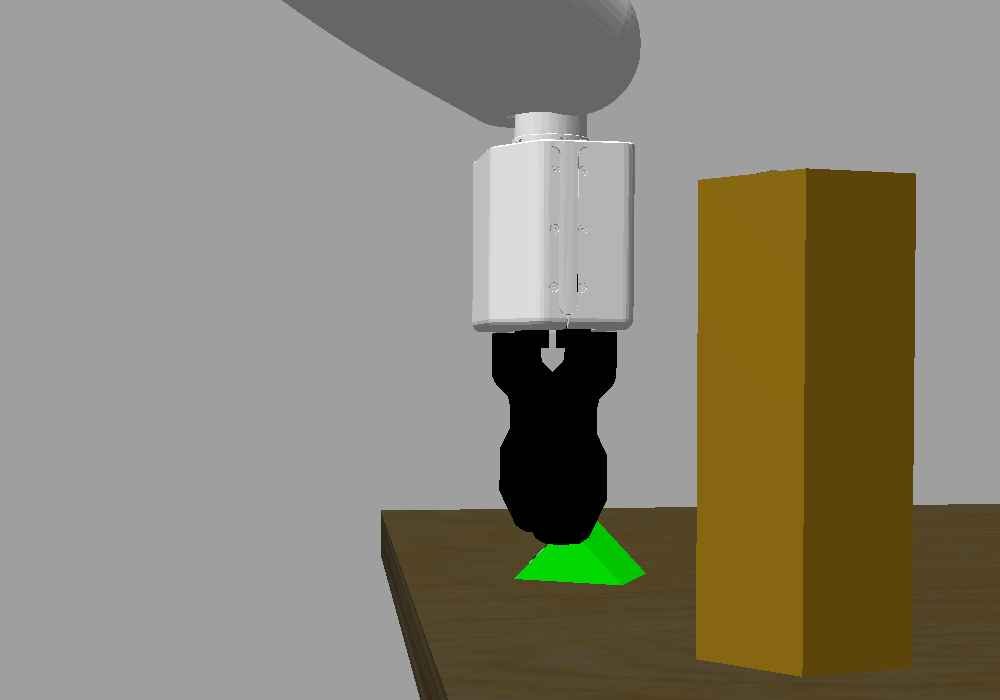
\includegraphics[scale = 0.18]{images/manipulations/pickGreen.png}
            \captionof{figure}{Pick Green}
        \end{minipage}
    \end{figure}           
    
    \item Finally, we decided to use different approach distances to grasps the different object, i.e. :
        \begin{itemize}
            \item for the Blue Hexagon, we modified the actual pick pose, by :
            \begin{itemize}
                \item subtracting on the x axis of the pick pose \\ $GRIPPER\_LENGTH + (HEXAGON\_DIAMETER / 2.0) + offset$ \\ where offset is equal to 0.1 (10 cm);
                \item adding on the z axis of the pick pose $HEXAGON\_HEIGHT / 3.0$;
            \end{itemize}
            \begin{center}
            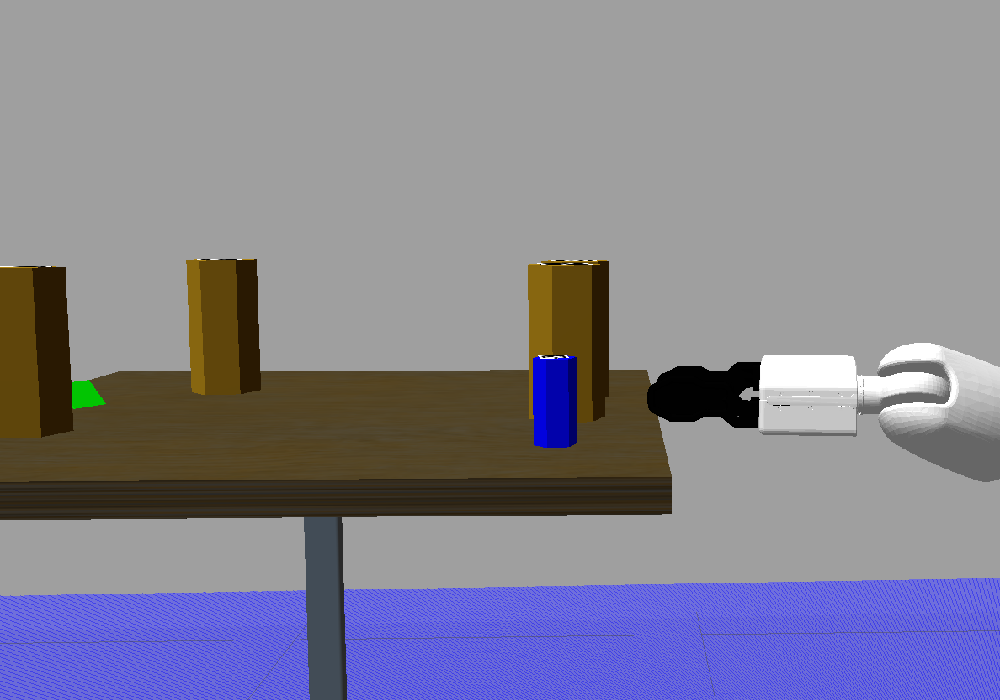
\includegraphics[scale = 0.3]{images/manipulations/approBlue.png}    
            \end{center}
            \item for the Green Tetrahedron, we modified the actual pick pose, by :
            \begin{itemize}
                \item adding on the z axis of the pick pose \\ $GRIPPER\_LENGTH + (TRIANGLE\_HEIGHT / 2.0) + offset)$ \\ where offset is equal to 0.1 (10 cm);
            \end{itemize}        
            \begin{center}
            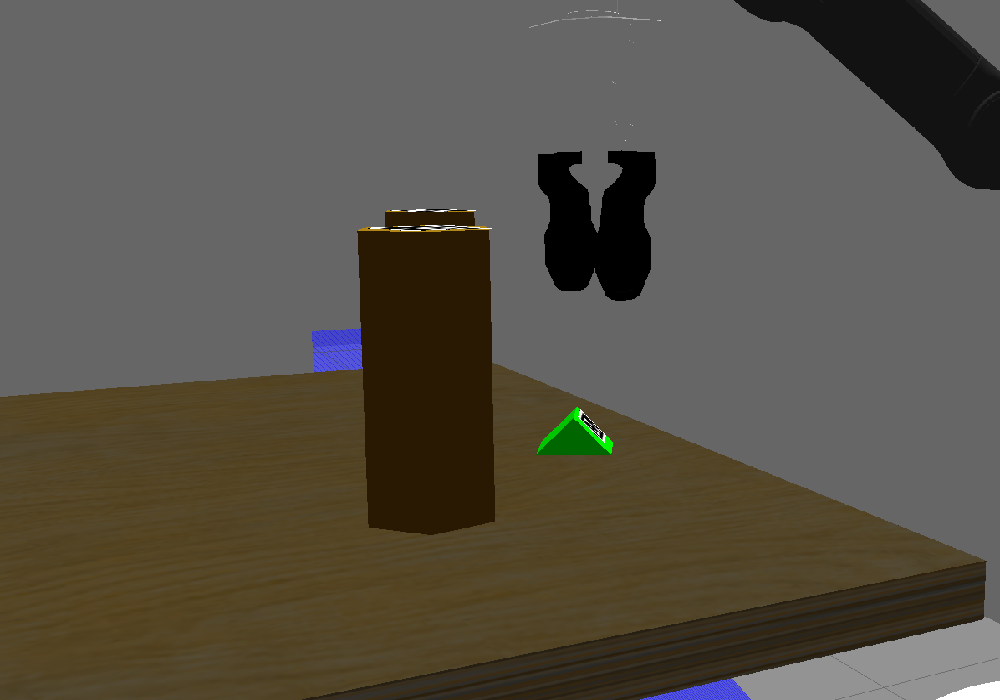
\includegraphics[scale = 0.3]{images/manipulations/approGreen.png}    
            \end{center}
            \item for the Red Cube, we modified the actual pick pose, by :
            \begin{itemize}
                \item adding on the z axis of the pick pose  $GRIPPER\_LENGTH + offset$ where offset is equal to 0.1 (10 cm);
            \end{itemize}            
            \begin{center}
            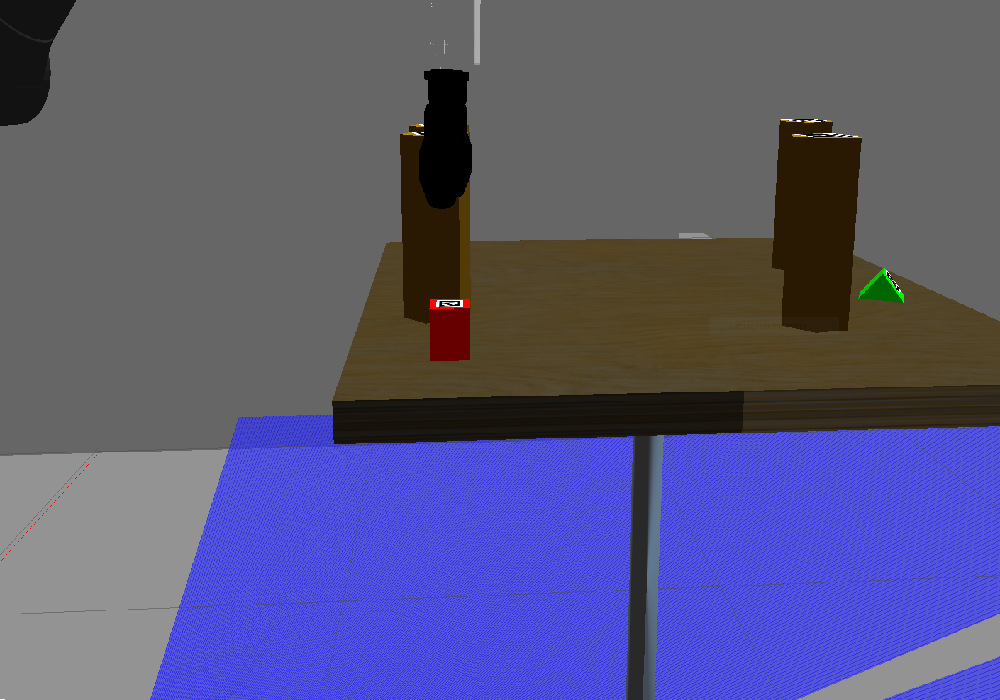
\includegraphics[scale = 0.3]{images/manipulations/approRed.png}    
            \end{center}
        \end{itemize}    
\end{enumerate}    

\subsection{Detection Assumptions}
During the detection of : 
\begin{itemize}
    \item the position of the pick-table;
    \item the position of the objects on the pick-table;    
\end{itemize}
we have assumed that the robot is placed in one of the picking positions i.e. either \textbf{\textcolor{red}{red}}, \textbf{\textcolor{blue}{blue}} or \textbf{\textcolor{ForestGreen} {green}} positions (as illustrated before in the Navigation Assumption part) and is already lifted up. With these assumptions we can assume that the pick-table is in front of the robot and, in order to look at it, the robot has to move the head a little bit.